\documentclass[12pt,a4paper]{report}
\usepackage[a4paper,margin=1in]{geometry}
\usepackage{graphicx}
\usepackage{lmodern}
\usepackage{setspace}
\usepackage{titlesec}
\usepackage{lipsum}
\usepackage{fancyhdr}
\usepackage[Sonny]{fncychap}

%--------------------------------
% Chapter Title
%--------------------------------
\ChNameVar{\raggedleft\bfseries\Large}   % "CHAPTER" word
\ChNumVar{\raggedleft\bfseries\Large}    % Chapter number
\ChTitleVar{\raggedleft\bfseries\Large}  % Chapter title

%--------------------------------
% Section Title
%--------------------------------
\titleformat{\section}[block]
    {\titlerule[2pt]\addvspace{0.8ex}%
    \bfseries\Large}
    {\thesection}{0.5em}
    {}[{\addvspace{0.4ex}\titlerule[2pt]}]
\titlespacing{\section}{0pt}{*4}{*4}

% Display current section in header:
\pagestyle{fancy}
\fancyhf{}
\fancyhead[L]{\nouppercase{\rightmark}}
\fancyfoot[C]{\thepage}

\begin{document}

% Title Page
\begin{titlepage}
    \centering
    
    % University logo at the top
    
\includegraphics[width=0.3\textwidth]{images/uantwerp_logo.png}\\[1cm]
    
    {\Huge \textbf{Multimodal Data Integration for Predictive Modelling of Measles Vaccine Response with Cross-Vaccine Marker Validation}} \\
    \vfill
    
    {\Large \textbf{Elias Dams}}\\[1cm]
    
    \textbf{Promotor:} Dr. Pieter Meysman\\
    \textbf{Supervisor:} Fabio Affaticati\\[1.5cm]
    
    {\Large \textbf{University of Antwerp}}\\
    {\large Faculty of Science}\\[0.5cm]
    
    \textbf{2024-2025}\\[1.5cm]
    
    Submitted in fulfilment of the requirements for the degree of\\
    \textbf{Master in Computer Science: AI \& Data Science}\\[1cm]
    
    \textbf{June 2025}\\[2cm]
    
    % Decorative line at the bottom
    \vfill
    
\includegraphics[width=1.0\textwidth]{images/bottom_design.jpg}

\end{titlepage}

% Table of Contents
\tableofcontents
\newpage

% List of Figures, Tables, Acronyms
\listoffigures

\listoftables

\chapter*{List of Acronyms}
- TCR: T-cell receptor

% Preliminary Sections
\chapter*{Summary}

\chapter*{Acknowledgements}

\chapter*{Abstract}


% Chapters
\chapter{Introduction}
...

\chapter{Background}

I will give some background about topics that should be understood of 2 diciplines to understand the thesis. 

\section{Background in Biology}

\subsection{Immune System Overview}

\begin{figure}[htbp]
  \centering
  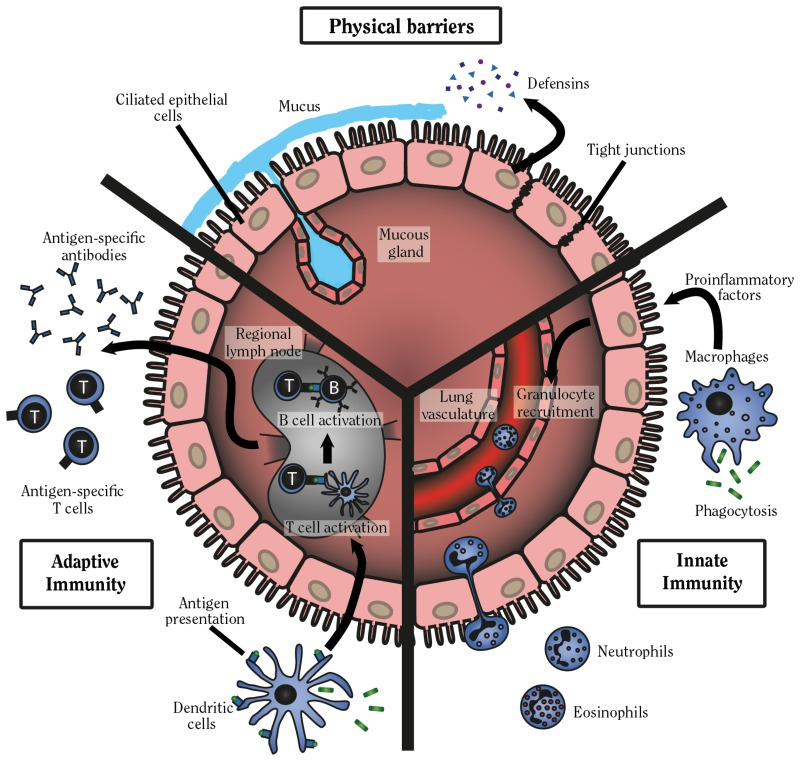
\includegraphics[width=0.8\textwidth]{images/Diagram_of_innate_and_adaptive_immunity.jpg} % your image file
  \caption[Diagram of Innate and Adaptive Immunity]{Diagram showing physical barriers, innate immune cells (e.g., macrophages, dendritic cells, natural killer cells) and adaptive immune components (B and T cells) working together. Reproduced from Figure 10.5 in \emph{The Health Consequences of Smoking—50 Years of Progress: A Report of the Surgeon General} (2014) \cite{smoking2014}.}
  \label{fig:immunity}
\end{figure}

First of all, I would like to give an overview of how the immune system works. The immune system can be roughly divided into three main parts, as depicted in Figure \ref{fig:immunity}:\\
\\
\textbf{Physical barriers (top)}\\
Physical barriers such as the skin and mucous membranes form the body’s first line of defense by preventing most pathogens from entering.\\
\\
\textbf{Innate Immunity (right)}\\
In case a pathogen still crosses the barriers, innate immunity comes into action. This defense is rapid and non-specific. Think of macrophages and neutrophils as cells that engulf invaders through a process called phagocytosis. Eosinophils and other granulocytes also attack pathogens or initiate inflammatory responses. Natural killer cells (NK cells) are also part of innate immunity and can directly destroy infected or abnormal cells. Although this response is very rapid, it does not recognize pathogens in the same specific way as the next branch. \cite{janeway2001immunobiology}\\
\\
\textbf{Adaptive Immunity (left)}\\
Acquired or adaptive immunity is the “slower but more targeted” defense. B cells are an important part here. They are responsible for producing antibodies, which are proteins that bind to specific antigens (foreign substances) to neutralize or mark them for destruction. The level of these antibodies in the blood is often measured as “antibody titers". Higher titers generally indicate a stronger immune response. T cells are also crucial and have several roles. They help coordinate the immune response (often referred to as “helper T cells”) and can directly kill infected cells (cytotoxic T cells). T cell receptors (TCRs) are highly specific and can be sequenced to understand which T cell clones are active in response to a vaccine. A major advantage of adaptive immunity is that it “learns” from previous exposure, allowing for much faster and more powerful immune responses in the event of repeated infection. This ability to form memory also underlies how vaccines work. \cite{janeway2001immunobiology}\\
\\
Together, these three pillars provide a robust defense system that is able to successfully ward off or fight off most infections. It is also this dynamic between innate and adaptive immunity that determines the degree of vaccine response. the innate branch prepares the way, while the adaptive branch provides targeted antibodies and memory cells. This is important to understand because my models integrate elements of both the innate and adaptive immune systems. For example, innate markers such as cytokine levels and certain cell counts (measured via cytometry) can provide early signals about the body's general readiness to respond. Meanwhile, adaptive markers, such as TCR sequences of T cells, directly reflect the specific immune response that leads to antibody production after vaccination. Combining this data gives us a more complete picture of the immune landscape, allowing me to better predict how effectively an individual will respond to the measles vaccine.

\subsection{Antibody Titers }
In addition to assessing the cellular components of the immune response, it is crucial to quantify the functional output of the adaptive immune system, namely antibody production. Antibody titers provide a quantitative measurement of the concentration of specific antibodies in the blood, and essentially reflect the “signal strength” of the immune response against a particular antigen. High titers usually mean that the immune system is actively fighting off the pathogen by targeting and clearing it effectively. In contrast, low titers indicate a weaker response and thus less robust protection.\\
\\
To determine antibody titers in the laboratory, serial dilution tests are often used. In these tests, a serum sample is progressively diluted and each dilution tests its ability to bind to the target antigen. The titer is defined as the highest dilution at which antibodies can still be detected. This method allows a practical estimate of the antibody concentration in the original sample.\\
\\
In my research thesis, antibody titers serve as an important biomarker to label vaccine response categories. By categorizing individuals based on their antibody titers, I can distinguish between strong and weak responders. This classification is essential for developing and validating predictive models because it provides a clear, quantifiable endpoint that reflects the effectiveness of the measles vaccine in eliciting a protective immune response.

\pagebreak
\section{Background in Computer science}
...

\bibliographystyle{plain}
\bibliography{references}

\end{document}
